%%
%% Copyright 2007, 2008, 2009 Elsevier Ltd
%%
%% This file is part of the 'Elsarticle Bundle'.
%% ---------------------------------------------
%%
%% It may be distributed under the conditions of the LaTeX Project Public
%% License, either version 1.2 of this license or (at your option) any
%% later version.  The latest version of this license is in
%%    http://www.latex-project.org/lppl.txt
%% and version 1.2 or later is part of all distributions of LaTeX
%% version 1999/12/01 or later.
%%
%% The list of all files belonging to the 'Elsarticle Bundle' is
%% given in the file `manifest.txt'.
%%
%% Template article for Elsevier's document class `elsarticle'
%% with harvard style bibliographic references
%% SP 2008/03/01
%%
%%
%%
%% $Id: elsarticle-template-5-harv.tex 159 2009-10-08 06:08:33Z rishi $
%% $URL: http://lenova.river-valley.com/svn/elsbst/trunk/elsarticle-template-5-harv.tex $
%%
\documentclass[preprint,authoryear,12pt]{elsarticle}
\usepackage{setspace}
%% \doublespacing
%% Use the option review to obtain double line spacing
%% \documentclass[authoryear,preprint,review,12pt]{elsarticle}

%% Use the options 1p,twocolumn; 3p; 3p,twocolumn; 5p; or 5p,twocolumn
%% for a journal layout:
%% \documentclass[final,authoryear,1p,times]{elsarticle}
%% \documentclass[final,authoryear,1p,times,twocolumn]{elsarticle}
%% \documentclass[final,authoryear,3p,times]{elsarticle}
%% \documentclass[final,authoryear,3p,times,twocolumn]{elsarticle}
%% \documentclass[final,authoryear,5p,times]{elsarticle}
%% \documentclass[final,authoryear,5p,times,twocolumn]{elsarticle}

%% if you use PostScript figures in your article
%% use the graphics package for simple commands
%% \usepackage{graphics}
%% or use the graphicx package for more complicated commands
\usepackage{graphicx, subfigure}
\usepackage{caption}
%% or use the epsfig package if you prefer to use the old commands
%% \usepackage{epsfig}

%% The amssymb package provides various useful mathematical symbols
\usepackage{amssymb}
%% The amsthm package provides extended theorem environments
%% \usepackage{amsthm}

%% The lineno packages adds line numbers. Start line numbering with
%% \begin{linenumbers}, end it with \end{linenumbers}. Or switch it on
%% for the whole article with \linenumbers after \end{frontmatter}.
%% \usepackage{lineno}

%% natbib.sty is loaded by default. However, natbib options can be
%% provided with \biboptions{...} command. Following options are
%% valid:

%%   round  -  round parentheses are used (default)
%%   square -  square brackets are used   [option]
%%   curly  -  curly braces are used      {option}
%%   angle  -  angle brackets are used    <option>
%%   semicolon  -  multiple citations separated by semi-colon (default)
%%   colon  - same as semicolon, an earlier confusion
%%   comma  -  separated by comma
%%   authoryear - selects author-year citations (default)
%%   numbers-  selects numerical citations
%%   super  -  numerical citations as superscripts
%%   sort   -  sorts multiple citations according to order in ref. list
%%   sort&compress   -  like sort, but also compresses numerical citations
%%   compress - compresses without sorting
%%   longnamesfirst  -  makes first citation full author list
%%
%% \biboptions{longnamesfirst,comma}

% \biboptions{}

%% My Macros
\newcommand{\specialcell}[2][c]{
  \begin{tabular}[#1]{@{}c@{}}#2\end{tabular}}

\journal{Cognition}

\begin{document}

\begin{frontmatter}

%% Title, authors and addresses

%% use the tnoteref command within \title for footnotes;
%% use the tnotetext command for the associated footnote;
%% use the fnref command within \author or \address for footnotes;
%% use the fntext command for the associated footnote;
%% use the corref command within \author for corresponding author footnotes;
%% use the cortext command for the associated footnote;
%% use the ead command for the email address,
%% and the form \ead[url] for the home page:
%%
\title{Learning grammatical categories using paradigmatic
  representations: Substitute words for language acquisition}

\author[rvt]{Mehmet Ali Yatbaz\corref{cor1}}
\ead{myatbaz@ku.edu.tr}
\author[rvt]{Volkan Cirik}
\ead{vcirik@ku.edu.tr}
\author[rvt]{Deniz Yuret}
\ead{dyuret@ku.edu.tr}

\cortext[cor1]{Corresponding author. Address: Department of Computer
  Engineering, Ko\c{c} University, 34450, Istanbul, Turkey}

\address[rvt]{Ko\c{c} University, Istanbul, Turkey}


%% .}

%% \tnotetext[label1]{}
%% \author{Name\corref{cor1}\fnref{label2}}
%% \ead{email address}
%% \ead[url]{home page}
%% \fntext[label2]{}
%% \cortext[cor1]{}
%% \address{Address\fnref{label3}}
%% \fntext[label3]{}

%% \title{}

%% use optional labels to link authors explicitly to addresses:
%% \author[label1,label2]{<author name>}
%% \address[label1]{<address>}
%% \address[label2]{<address>}

\begin{abstract}
%% Text of abstract
We study the paradigmatic representations of contexts for 
grammatical category acquisition in child directed speech. 
Learning syntactic categories is an essential task in language
acquisition. Previous studies show that co-occurrence
patterns or distributional knowledge could be handy
for this task. These studies usually use co-occurrences of the preceding and following words
to group words. However, the neighbouring words, or frames, are not able
to exchange information when there is not enough overlapping
between frames. In this work, we propose to use paradigmatic representations of words which
are the probable substitutes of words instead of frames.
Our experiments on child directed speech show that the probable substitutes are better than
frames in terms of accuracy and robust in terms of the parameters on which
they depend.

\end{abstract}

\begin{keyword}
Language acquisition \sep Grammatical categorization \sep
Distributional information \sep Corpus analysis \sep Computational
modeling \sep Paradigmatic approach
%% keywords here, in the form: keyword \sep keyword
%% MSC codes here, in the form: \MSC code \sep code
%% or \MSC[2008] code \sep code (2000 is the default)

\end{keyword}

\end{frontmatter}

% \linenumbers
%% main text
\section{Introduction}
\label{sec:introduction}
\subsection{Psycholinguistic evidence relevant to substitutes}

\subsection{Comparison with previous distributional approaches}

Following two examples\footnote{These examples are extracted from the Anne
corpus and substitute probabilities are calculated as described in
Section~\ref{sec:substitute_vectors}.} illustrate the advantage of paradigmatic
representations in uncovering similarities where no overt similarity that can
be captured by a syntagmatic representation exists. The word ``you'' from the
first sentence and the word ``I'' from the second sentence have no common
neighbors.  The paradigmatic representation captures the similarity of these
words by suggesting the same top substitutes for both (the numbers in
parentheses give substitute probabilities): 

\begin{quote}
  \small
  % Anne corpus sentence id:13228
  (1) \noindent{\em ``they fall out when {\bf you} put it in the box .''}\\
  \noindent{\bf you:} you(.8188), I(.1027), they(.0408), we(.0146) $\ldots$
\end{quote}

\begin{quote}
  \small
  % Anne corpus sentence id: 13085
  (2) \noindent {\em ``what have {\bf I} got here ?''}\\
  \noindent {\bf I:} we(.8074), you(.1213), I(.0638), they(.0073) $\ldots$
\end{quote}

The high probability substitutes reflect both semantic and syntactic properties
of the context.  Top substitutes for ``I'' and ``you'' are not only nouns, but
specifically nouns compatible with the semantic context.  Top substitutes for
the word ``fall'' in the first example consist of words that are also  verbs:
come(.7875), go(.0305), fall(.0232), were(.0187) $\ldots$.



\section{Related Work}
Previous research demonstrate that infants have a mechanism to process
statistical properties of natural language(Saffran et al., 1996).
Distributional knowledge,which is also a statistical approach to natural
language, refers to the notion that context of a word determines grammatical
properties of it. For instance, (Gomez, 2002) and (Van Heugten et al.,2010)
demonstrated that distributional statistics help infants acquire non-adjacent
dependencies. Distributional knowledge also plays an important part in word
segmentation task(Saffran,Newport, et al., 1996).

One of the approaches of distributional information to construct syntactic
categories is the work of (Redington et al., 1998). They define the context of
a word as previous and following words. With this definition, they construct
context vectors of target words for clustering. Using average link clustering
with a treshold maximizing accuracy and completeness, target  words are
seperated into categories. Although the categorizations are generally accurate,
the method lacks of completeness. Furthermore, as (Ambridge  and 2011) pointed
out one might question what could be the underlying process to determine the
treshold for infants to do such clustering.

(Cartwight et al.,1997) introduces an incremental method to make use of
distributional knowledge. Intrinsic idea behind the method is that no language
learner has ever a chance to process all the sentences of the language to learn
syntactic categorization, thus, a generalization method such as distributional
processing may help learner confine the search space for later generalization.
To accomplish this, they convert the problem into Minimum Descriptive Language
optimization problem. The crucial part of the method is that after a sentence
is processed, it is forgotton. Results are similar with Redingtons's work, high
in accuracy but low in completeness. Still, it shows that distributional
knowledge is powerful for syntactic categorization even if the learner is
exposed the small amount of syntactic knowledge of the language.

By extending the work on adults with artificial language inputs (Mintz,2002),
(Mintz, 2003) proposes a notion to represent the context of a word. Frequent
frames can be defined as two jointly appearing words with one word in the
middle. Experiments on child directed speech reveal that even relatively small
fraction of frames has ability to categorize the half of the corpora. Though
the accuracy is impressive, the same as previous work, it suffers from
completeness, in addition, it has covarege problem. As a further step, (St.
Clair et al., 2010), combines the bigram's coverage power(Redington et
al.,1998),(Monaghan and Christansen, 2008) and accuracy of fixed
frames(Mintz,2003). Extensive experiments result that infants make use of both
bigram and trigram sources. As they pointed out, they may even use higher-order
relationships among words. 


(Freudenthal et al.,2004) points out a different complication on distributional
methods for constructing syntactic categories. One of the core ideas behind
distributional methods is that words in the same context share the same
syntactic categories and can be used interchangebly(REFERENCE HERE).
Freudenthal claims that evaluation methods used in previous work such as
(Mintz, 2003), (Cartwright, 1997) and (Redington et al., 1998) can be
misleading. In those work, if a word is substituted with another one in its
category, the resulting sentences erronous in a way that are not observed in
infants speech. As a success criteria, they argue that proposed categorization
should generate plausible sentences. They introduce chunking mechanism to
overcome this problem by merging  words that are seen frequently. Results seems
successful to generate meaningful sentences after substitution, still, the
proposed solution is computationally complex to disclose the learning mechanism
in infants.



\section{Substitute Words}
\label{sec:substitute_vectors}

In this study, we predict the syntactic category of a word in a given
context based on its most likely substitute words.  Note that the
substitute word distribution is a function of the context only and is
indifferent to the target word.

\cite{20674613} demonstrated that learning left and right bigrams
together was much more effective than learning them individually.
Thus it is best to use both the left and the right context when
estimating the probabilities for potential lexical substitutes.  For
example, in \emph{``He lived in San Francisco suburbs.''}, the token
\emph{San} would be difficult to guess from the left context but it is
almost certain looking at the right context.  We define $c_w$ as the
$2n-1$ word window centered around the target word position: $w_{-n+1}
\ldots w_0 \ldots w_{n-1}$.  The probability of a substitute word $w$
in a given context $c_w$ can be estimated as:
\begin{eqnarray}
  \label{eq:lm1}P(w_0 = w | c_w) & \propto & P(w_{-n+1}\ldots w_0\ldots w_{n-1})\\
  \label{eq:lm2}& = & P(w_{-n+1})P(w_{-n+2}|w_{-n+1})\ldots P(w_{n-1}|w_{-n+1}^{n-2})\\
  \label{eq:lm3}& \approx & P(w_0| w_{-n+1}^{-1})P(w_{1}|w_{-n+2}^0)\ldots P(w_{n-1}|w_0^{n-2})
\end{eqnarray}
where $w_i^j$ represents the sequence of words $w_i w_{i+1} \ldots
w_{j}$.  In Equation \ref{eq:lm1}, $P(w|c_w)$ is proportional to
$P(w_{-n+1}\ldots w_0 \ldots w_{n+1})$ because the words of the
context are fixed.  Terms without $w_0$ are identical for each
substitute in Equation \ref{eq:lm2} therefore they have been dropped
in Equation \ref{eq:lm3}.  Finally, because of the Markov property of
n-gram language model, only the closest $n-1$ words are used in the
experiments.

Near the sentence boundaries the appropriate terms were truncated in
Equation \ref{eq:lm3}.  Specifically, at the beginning of the sentence
shorter n-gram contexts were used and at the end of the sentence terms
beyond the end-of-sentence utterance were dropped.  

%% Rest of this section details the choice of the data set, the
%% vocabulary and the estimation of substitute probabilities.
%% For computational efficiency only the top 100 substitutes and their
%% unnormalized probabilities were computed for each of the 1,173,766
%% positions in the test set\footnote{The substitutes with unnormalized
%%   log probabilities can be downloaded from
%%   \mbox{\url{http://goo.gl/jzKH0}}.  For a description of the {\sc
%%     fastsubs} algorithm used to generate the substitutes please see
%%   \mbox{\url{http://arxiv.org/abs/1205.5407v1}}.  {\sc fastsubs}
%%   accomplishes this task in about 5 hours, a naive algorithm that
%%   looks at the whole vocabulary would take more than 6 days on a
%%   typical 2012 workstation.}.  The probability vectors for each
%% position were normalized to add up to 1.0 giving us the final
%% substitute vectors used in the rest of this study.

% what is the LM training data
%Train => 5181717 126019973 690121813

To compute substitute probabilities we trained a language model using
approximately 6.8 million tokens of child-directed speech data from
the CHILDES corpus \citep*{macwhinney2000childes} (excluding sections of
[test-set])
% how is the language model trained
We used SRILM \citep*{Stolcke2002} to build a 4-gram language model with
Kneser-Ney discounting.
% what is the vocabulary
Words that were observed less than 2 times in the LM training data
were replaced by \textsc{unk} tags, which gave us a vocabulary size of
21734.
% what is the test data
[What is the test data? Where should we put this?]
%% The first 24,020 tokens of the Penn Treebank Wall Street Journal
%% Section 00 (PTB24K) was used as the test corpus to be induced.  The corpus
%% size was kept small in order to efficiently compute full distance
%% matrices.  Substitution probabilities for 12,672 vocabulary words were
%% computed at each of the 24,020 positions.
% perplexity
[perplexity]
%% The perplexity of the 4-gram language model on the test corpus was
%% 55.4 which is quite low due to using a small 
%% vocabulary and in-domain data.
% what is the tag set

%% Experiment Section Counter
\newcounter{ExperimentCounter}
\setcounter{ExperimentCounter}{1}
\section{Experimental Setup}

In this section we explain the experimental setup we used. First we
demonstrate how we process the input corpora. Secondly, we present
the parameters used to train a language model and calculate substitute word
probabilities. Lastly, we clarify the grammatical categories used for evaluation.

\subsection{Input Corpora}

In order to obtain comparable results with \cite{clair2010} and
\cite{Mintz200391}, we use the same six corpora of child-directed speech from
the CHILDES\footnote{ Specifically, CHILDES version $2.0.1$ is used in
experiments.} corpus \citep*{macwhinney2000childes}: Anne and Aran
\citep*{theakston2001role}, Eve \citep*{JCL:1765112}, Naomi
\citep*{sachs1983talking}, Nina \citep*{suppes1974semantics}, Peter
\citep*{Bloom1974380, bloom1975structure}.  Following \cite{Mintz200391} we
only analyze the adult utterances in sessions where the target child is 2.6
years old or younger.  Prior to the analysis, we perform the data preprocessing
detailed in \ref{app:preprocessing}.

% \subsubsection{Target Words}
%% How do we extract frames? Which words are the our target words
\begin{table}[ht]
  \centering
  \caption{Summary of the total number of tokens, utterances and types in each
  child corpus together with the number of utterances and types that are obserd
  as target word in $aXb$.}
  \begin{tabular}{lccccccc}
    \hline
    Corpus & Tokens & Utterances & \multicolumn{2}{c}{\specialcell{Utterances\\Categorized}} & Types & \multicolumn{2}{c}{\specialcell{Types\\Categorized}}\\
    \cline{4-5}
    \cline{7-8}
    & & & Count & \% & & Count & \% \\
    \hline
    Anne & 121726 & 93371 & 42789 & 45.82 & 2623 & 1846 & 70.37\\ 
    Aran & 129823 & 104997 & 54768 & 52.16 & 3256 & 2595 & 79.69\\ 
    Eve & 78778 & 59095 & 27315 & 46.22 & 2184 & 1465 & 67.07\\
    Naomi & 38302 & 28793 & 13002 & 45.15 & 1883 & 1194 & 63.40\\
    Nina & 89957 & 72879 & 39335 & 53.97 & 2036 & 1580 & 77.60\\
    Peter & 94521 & 72834 & 34997 & 48.05 & 2145 & 1472 & 68.62\\
    \hline
  \end{tabular}
  \label{tab:corpusstat}
\end{table}
 
Word sequences that consist of three words and do not contain any utterance
boundaries are extracted from each child corpus separately
\citep*{Mintz200391}.  The first and the third words of sequences are treated
as frame elements while the middle utterance is the target word that is
categorized.  Table~\ref{tab:corpusstat} summarizes the number of target word
tokens and types in each corpus.   

To calculate substitutes we extracted the 4-gram left and right contexts of
each target word when they are available \footnote{Lower order n-gram contexts
are extracted when the 4-gram left or right context is not available.}.

\subsubsection{Language Modeling for Substitute Words}
\label{s:lm}
We extracted training data of approximately 6.8 million tokens\footnote{Anne,
Aran, Eve, Naomi and Peter corpora are excluded.} of child-directed speech data
from CHILDES following the steps defined in Section~\ref{app:preprocessing}.
To calculate substitute word probabilities, we train a 4-gram language model with
Kneser-Ney discounting on the training data using SRILM \citep*{Stolcke2002}.
Words that were observed less than 2 times in the language model training data
were replaced with unknown word tag \textsc{<unk>}, which gave us a vocabulary
size of 21734.

\subsubsection{Grammatical categories and Evaluation}
The grammatical category of words in CHILDES are extracted by first
applying the MOR parser \citep*{macwhinney2000childes} and then using
the POST disambiguator \citep*{sagae2004automatic}.  The accuracy of
CHILDES grammatical categories is approximately 95\%
\citep*{parisse2000automatic} and it is encoded in the MOR line of the
CHILDES corpus.

To evaluate classification accuracy we use the standard labeling
\citep*{Mintz200391}\footnote{\cite{Mintz200391} also defined an expanded
labeling in which pro-nouns, auxiliaries and copula forms have their own
categories.} that categorizes target words as: nouns (including pronouns), verbs
(including copula and auxiliaries forms), prepositions, adjectives, adverbs,
determiners, conjunctions, wh-words, negation (i.e., ``not'') and
interjections.


%% Define frames in here again? also in related work.
%% What is standard labeling? 
%% Are we going to report accuracy and completeness

\subsection{Computational Modeling Algorithm}
\label{s:computational}
% Why do we choose feedforward connectionist model?
\cite{clair2010} used a feed-forward connectionist model to compare
the effect of distributional cues from various frame types on the
grammatical category learning.  We adopt their framework to compare the
paradigmatic representation (substitute words) with the best performing
syntagmatic representation (i.e., flexible frames).
% What are the input and output layer
% What does the connectionist model do? Briefly explain without giving
% too much mathematical details
% Two aspects:  
% description of learning process
% how to represent distributional

A prototypical connectionist model consists of input, hidden and
output layers.  Input and output layers are connected to each other
through the hidden layer.  The behavior of the output units are
determined by the activity of the hidden layers which is triggered by
the input layer.

% How do they represent the frame/input information?
We train separate connectionist models to compare flexible frames ($aX+Xb$) to
the substitute words ($a*b$).  For each model we input the distributional
information to the feed-forward connectionist model in the following way,

\begin{itemize}
%#\item $aXb$: Each input unit represents a distinct frame thus only one
% unit is activated (i.e. set to 1) for each target word.
\item {\bf$aX+Xb$ model:} The first and second half of the input units
  correspond to the preceding bigram ($a$) and the succeeding bigram
  ($b$), respectively.  Thus two input units are activated for each
  target word.
\item {\bf $a*b$ model:} Each input unit represents a distinct
  substitute and input units that correspond to the substitutes of the
  target word are set to the number of their occurrences in the
  sampled substitute set.
\end{itemize}

\begin{figure}[ht]
  \centering
  \includegraphics[width=.6\textwidth]{../figures/inputlayer.pdf}
  \caption{Number of input layer units of the flexible frame ($aX + Xb$) and
    the substitute based model($a*b$) are summarized.  $a*b$ samples 16
    substitutes per target word.  Standard errors are reported with error bars. 
  }
  \label{fig:inputunits}
\end{figure}
Table~\ref{fig:inputunits} presents the number of input layer units of
syntagmatic and paradigmatic representation based models on each child
corpus seperately.  The number of distinct frames is fixed for any
given corpus while the number of distinct substitutes varies due to
the random sampling.

% Give an example sentence to show how we represent each frame
Each output unit represents a distinct grammatical category therefore the
models are expected to produce only one active (non-zero) output unit for each
target word.  If there are more than one active units present in the output
layer\footnote{why neural network produces more than one active unit.}, the
target word is assigned to the corresponding grammatical category of the output
unit with the largest value.

Both models have 10 output units due to the standard labeling
\citep*{Mintz200391}.

Unless stated otherwise, all connectionist models in this paper uses the
following parameters: (1)number of hidden units is set to 200 and initialized
randomly for each model, (2){\bf backprobagation(0.1)}, (3){\bf learning
rate},(4) {\bf sigmoid...}

\subsection{Training and Testing}
\label{sec:training}
%%% How do we split the train and test
% 10-fold cross valdiation
% -> define/implementaion
% -> advantage

We measure and compare the classification accuracy of models by applying
10-fold cross validation on the union of six child corpora.  To perform 10-fold
cross validation we randomly split each child corpus into 10 folds.  At each
iteration a single fold from each child corpus is kept as the test data while
the union of remaining 9 folds of each child corpus are used as the training
data.  We repeat this process until all folds are used exactly once as the test
data and report the average accuracy of 10 runs on each child corpus
separately.  The main advantage of the cross validation is that all sentences
are eventually used both for testing and training. [!! cite]

To compare the effects of paradigmatic representation ($a*b$) with the
syntagmatic one ($aX+Xb$) we train and test both models using the identical
10-fold cross validation split.  Thus every model in this paper exposed to the
identical sequence of training and testing patterns.  Unless stated otherwise,
in the rest of this paper, we stopped the training phase of feed-forward
connectionist model on each corpus after $100K$ input patterns, used the
standard labeling to evaluate model accuracies, calculated substitute
distributions with with the language model defined in Section~\ref{s:lm} and sampled 16
substitutes per target word in models using the paradigmatic representation.

In the next section we replicate the corpus analysis of \cite{Mintz200391} and
\cite{clair2010}.  Section~\ref{s:exp_paradigmatic} compares the classification
accuracies of syntagmatic and paradigmatic representation based models.  The
effects of the number of substitutes and the language model n-gram order on the
paradigmatic model performance are inspected in Section~\ref{s:exp_substitutes}
and \ref{s:exp_ngram}, respectively. 

\section{Experiment \arabic{ExperimentCounter}: Syntagmatic vs Paradigmatic}
\label{s:exp_paradigmatic}
\stepcounter{ExperimentCounter}

In order to compare the distributional information of syntagmatic and
paradigmatic representations we train separate feed-forward connectionist
models for each child corpus based on these representations.  \cite{clair2010}
showed that flexible frames have richer distributional information than other
frame types both in terms of classification accuracy and coverage .  Thus we
only report results of the models based on substitute words ($a*b$) and
flexible frames ($aX+Xb$)\footnote{We can put the comparison with other frames
in Appendix.}. 

\subsection{Method} 
All models are trained and evaluated according to steps summarized in
Section~\ref{sec:training}.  Similar to analysis in \cite{clair2010}, we split
the training phase of each model into two as short and long training phases in
which we stop and evaluate the models on the corresponding test sets after
presenting identical 10K and 100K training patterns, respectively.  

\subsection{Results of Short Training Phase}
Table~\ref{t:framevssub10K} gives the overall classification accuracies of
$aX+Xb$ and $a*b$ models on each child corpus.  The accuracy of $a*b$ model
significantly outperforms the $aX+Xb$ model on each child corpora even with a
limited amount of training patters.  Lambdas of the $a*b$ model are
significantly closer to the perfect association than lambdas of the $aX+Xb$
model.  Lambdas of both models are significantly different from zero
association.
\begin{table}[ht]
  \small 
  \centering
  \caption{10-fold cross-validation classification accuracies of models based
    on flexible frames ($aX + Xb$) and substitutes ($a*b$) on each child corpus
    after 10K training patterns are summarized.  Standard errors are reported
    in parentheses.  Lambdas of $aX+Xb$ and $a*b$ are both tested against each
    other and zero association by using z-test.  All tests have $p<.001$.}
\begin{tabular}{lccccc}
    \hline
    Corpus & \multicolumn{2}{c}{$aX+Xb$} && \multicolumn{2}{c}{$a*b$} \\
    \cline{2-3}
    \cline{5-6}
    & Accuracy & $\lambda$ && Accuracy & $\lambda$\\
    \hline
%% With z-score differences    
%%    & Accuracy & $\lambda$ && Accuracy & $\lambda$ & $\lambda_{a*b}-\lambda_{aX+Xb}$\\
%%    \hline 
%%    Anne  & .6587 (.0255) & .4486 (.0365) && .7945 (.0126) & .6684 (.0301) & 6.02\\
%%    Aran  & .5618 (.0636) & .3332 (.0613) && .7814 (.0099) & .6500 (.0170) & 5.16\\
%%    Eve   & .6360 (.0230) & .4351 (.0359) && .8148 (.0095) & .7127 (.0142) & 7.73\\
%%    Naomi & .6191 (.0322) & .3907 (.0547) && .7917 (.0182) & .6673 (.0290) & 5.06\\
%%    Nina  & .6745 (.0245) & .4818 (.0384) && .8263 (.0124) & .7243 (.0188) & 6.31\\
%%    Peter & .6687 (.0238) & .4857 (.0293) && .8135 (.0139) & .7092 (.0209) & 7.62\\
    Anne  & .6587 (.0255) & .4486 (.0365) && .7945 (.0126) & .6684 (.0301)\\
    Aran  & .5618 (.0636) & .3332 (.0613) && .7814 (.0099) & .6500 (.0170)\\
    Eve   & .6360 (.0230) & .4351 (.0359) && .8148 (.0095) & .7127 (.0142)\\
    Naomi & .6191 (.0322) & .3907 (.0547) && .7917 (.0182) & .6673 (.0290)\\
    Nina  & .6745 (.0245) & .4818 (.0384) && .8263 (.0124) & .7243 (.0188)\\
    Peter & .6687 (.0238) & .4857 (.0293) && .8135 (.0139) & .7092 (.0209)\\
    \hline
  \end{tabular}
  \label{t:framevssub10K}
\end{table}

% \begin{table}[ht]
% \small
% \centering
% \caption{The 70\% of the sentences in the union of 6 child corpora are
%   used as the training set while the remaining 30\% sentences of each
%   corpus are used as the test set.  Average classification accuracy
%   (10 runs) of the supervised connectionist model for the standard
%   labelling on each child corpus after 10K words of training are
%   summarized and the corresponding standard errors are reported in
%   parentheses.}
% \begin{tabular}{|l|l@{ }|l@{ }|l@{ }|l@{ }|l@{ }|l@{ }|l@{ }|}
%   \hline
%   & \multicolumn{4}{c|}{Frames} & \multicolumn{2}{c|}{\specialcell{Number of \\ Substitute Words}}\\
%   \hline
%   Child & aX & Xb & aXb & aX + Xb & 1 & 16\\
%   \hline
%   Anne & .5317 (.0374)  & .5065 (.0214) & .3788 (.0279) & .6190 (.0253) & .6221 (.0333) & .7829 (.0059) \\
%   Aran & .5098 (.0344) & .4779 (.0171) & .5098 (.0289) & .5863 (.0227) & .5916 (.0371) & .7597 (.007) \\
%   Eve & .5408 (.036)  & .4905 (.0183) & .5408 (.0186) & .6125 (.0229) & .6189 (.0287) & .7862 (.0058) \\
%   Naomi & .5250 (.0269) & .4922 (.0205) & .3860 (.028) & .6019 (.0218) & .6021 (.0322) & .7672 (.0071) \\
%   Nina & .5412 (.0304) & .5032 (.0213) & .3950 (.0223) & .6308 (.0277) & .6474 (.0331) & .8089 (.0089) \\
%   Peter & .5359 (.036) & .5092 (.0216) & .5359 (.0188) & .6250 (.0252) & .6315 (.0263) & .7974 (.0082) \\
%   \hline
% \end{tabular}
% \end{table}

%%% Whole results
% \begin{table}[ht]
% \small
% \centering
% \caption{10 fold cross-validation accuracy of the connectionist model on each
%   child corpus with the standard labelling are summarized.  The training
%   phase of each corpus is stopped after 50K word patterns are presented.  Standard
%   errors are reported in parentheses.
% }

% \begin{tabular}{|c|c@{ }|c@{ }|c@{ }|c@{ }|c@{ }|c@{ }|c@{ }|}
%   \hline
%   & \multicolumn{4}{c|}{Frames} & \multicolumn{2}{c|}{\specialcell{Number of \\ Substitute Words}}\\
%   \hline
%   Child & aX & Xb & aXb & aX + Xb & 1 & 16\\
%   \hline
%   Anne & .6165 (.0119)  & .6150 (.0119) & .5251 (.0189) & .7545 (.0147) & .7321 (.0081) & {\bf .8273 (.0087)} \\
%   Aran & .5924 (.0193) & .5583 (.0193) & .4834 (.0131) & .7164 (.0151) & .7081 (.0074) & {\bf .8136 (.0096)} \\
%   Eve & .6337 (.0139)  & .5850 (.0116) & .5425 (.0198) & .7605 (.0104) & .7435 (.0208) & {\bf .8378 (.0199)} \\
%   Naomi & .6183 (.0165) & .5908 (.0254) & .5353 (.0234) & .7438 (.0156) & .7146 (.0136) & {\bf .8165 (.0147)} \\
%   Nina & .6353 (.0195) & .6097 (.0049) & .5556 (.0106) & .7745 (.0199) & .7527 (.0059) & {\bf .8494 (.0073)} \\
%   Peter & .6056 (.0205) & .6232 (.0205) & .5604 (.0115) & .7630 (.005) & .7398 (.0120) & {\bf .8437 (.0061)} \\
%   \hline
% \end{tabular}
% \end{table}
% \begin{table}[h]
% \label{tab:myfirsttable}
% \end{table}




To further investigate the accuracy gap between $aX+Xb$ and $a*b$ models, we
plot the classification accuracies of each grammatical category in the standard
labeling for both models in Figure~\ref{fig:category10K}.  Even after 10K
training patterns both models are able to achieve relatively higher accuracies
on nouns({\it n}), verbs({\it v}), determiners({\it det}) and prepositions({\it
prep}) than the rest of the grammatical categories.  The $a*b$ model is more
successful than the $aX+Xb$ model in learning grammatical categories such as
wh-words({\it wh}), adjectives({\it adj}), adverbs({\it adv}),
conjunctions({\it conj}) and negations({\it neg}). 

\begin{figure}[h]
  \subfigure[$aX+Xb$] {
    \includegraphics[width=0.5\textwidth]{../figures/fletags10K.pdf}
    \label{fig:subfig1}
  }
  \subfigure[$a*b$] { 
    \includegraphics[width=0.5\textwidth]{../figures/wsubtags10K.pdf}
    \label{fig:subfig2}
  }
 \caption{Individual tag accuracies of $aX+Xb$ and $a*b$ on each child corpus
 after $10K$ training patterns are presented.}
  \label{fig:category10K}
\end{figure}

Finally, with limited amount of training patterns the $a*b$ model is able to
categorize nine out of ten grammatical categories in each child corpus with
different levels of accuracies.  On the other hand, the $aX+Xb$ model performs
poorly on {\it wh}, {\it conj}, {\it adv}, {\it neg} and {\it int} and can not
correctly classify any members of these grammatical groups in at least one of
the child corpora.

\subsection{Results of Long Training Phase} 

Previous section shows that the $a*b$ model is more accurate than the $aX+Xb$
model on learning grammatical categories with limited amount of language
exposure.  In this section each model is trained with 100K input patterns to
observe the effect of extensive language exposure on learning.
\begin{table}[ht]
  \small
  \centering
  \caption{10-fold cross-validation classification accuracies of models based
    on flexible frames ($aX + Xb$) and substitutes ($a*b$) on each child corpus
    after 100K training patterns are summarized.  Standard errors are reported
    in parentheses.  Lambdas of $aX+Xb$ and $a*b$ are both tested against each
    other and zero association by using z-test.  All tests have $p<.001$.}
  \begin{tabular}{lccccc}
    \hline
    Corpus & \multicolumn{2}{c}{$aX+Xb$} && \multicolumn{2}{c}{$a*b$} \\
    \cline{2-3}
    \cline{5-6}
    & Accuracy & $\lambda$ && Accuracy & $\lambda$\\
%% With z-score differences    
%%    & Accuracy & $\lambda$ && Accuracy & $\lambda$ & $\lambda_{a*b}-\lambda_{aX+Xb}$\\
%%
%%    \hline
%%    Anne  & .7833 (.0072) & .6496 (.0118) && .8335 (.0078) & .7295 (.0123) & 6.49\\
%%    Aran  & .7495 (.0091) & .5991 (.0119) && .8218 (.0063) & .7147 (.0100) & 9.71\\
%%    Eve   & .7896 (.0073) & .6738 (.0106) && .8467 (.0113) & .7622 (.0172) & 5.13\\
%%    Naomi & .7643 (.0122) & .6232 (.0176) && .8212 (.0132) & .7140 (.0207) & 4.38\\
%%    Nina  & .8053 (.0083) & .6899 (.0148) && .8555 (.0058) & .7711 (.0082) & 5.48\\
%%    Peter & .7924 (.0083) & .6757 (.0126) && .8509 (.0083) & .7669 (.0090) & 7.23\\
    \hline
    Anne  & .7833 (.0072) & .6496 (.0118) && .8335 (.0078) & .7295 (.0123)\\
    Aran  & .7495 (.0091) & .5991 (.0119) && .8218 (.0063) & .7147 (.0100)\\
    Eve   & .7896 (.0073) & .6738 (.0106) && .8467 (.0113) & .7622 (.0172)\\
    Naomi & .7643 (.0122) & .6232 (.0176) && .8212 (.0132) & .7140 (.0207)\\
    Nina  & .8053 (.0083) & .6899 (.0148) && .8555 (.0058) & .7711 (.0082)\\
    Peter & .7924 (.0083) & .6757 (.0126) && .8509 (.0083) & .7669 (.0090)\\
    \hline
  \end{tabular}
  \label{t:framevssub100K}
\end{table}

% \begin{table}[ht]
% \small
% \centering
% \caption{The 70\% of the sentences in the union of 6 child corpora are
%   used as the training set while the remaining 30\% sentences of each
%   corpus are used as the test set.  Average classification accuracy
%   (10 runs) of the supervised connectionist model for the standard
%   labelling on each child corpus after 10K words of training are
%   summarized and the corresponding standard errors are reported in
%   parentheses.}
% \begin{tabular}{|l|l@{ }|l@{ }|l@{ }|l@{ }|l@{ }|l@{ }|l@{ }|}
%   \hline
%   & \multicolumn{4}{c|}{Frames} & \multicolumn{2}{c|}{\specialcell{Number of \\ Substitute Words}}\\
%   \hline
%   Child & aX & Xb & aXb & aX + Xb & 1 & 16\\
%   \hline
%   Anne & .5317 (.0374)  & .5065 (.0214) & .3788 (.0279) & .6190 (.0253) & .6221 (.0333) & .7829 (.0059) \\
%   Aran & .5098 (.0344) & .4779 (.0171) & .5098 (.0289) & .5863 (.0227) & .5916 (.0371) & .7597 (.007) \\
%   Eve & .5408 (.036)  & .4905 (.0183) & .5408 (.0186) & .6125 (.0229) & .6189 (.0287) & .7862 (.0058) \\
%   Naomi & .5250 (.0269) & .4922 (.0205) & .3860 (.028) & .6019 (.0218) & .6021 (.0322) & .7672 (.0071) \\
%   Nina & .5412 (.0304) & .5032 (.0213) & .3950 (.0223) & .6308 (.0277) & .6474 (.0331) & .8089 (.0089) \\
%   Peter & .5359 (.036) & .5092 (.0216) & .5359 (.0188) & .6250 (.0252) & .6315 (.0263) & .7974 (.0082) \\
%   \hline
% \end{tabular}
% \end{table}

%%% Whole results
% \begin{table}[ht]
% \small
% \centering
% \caption{10 fold cross-validation accuracy of the connectionist model on each
%   child corpus with the standard labelling are summarized.  The training
%   phase of each corpus is stopped after 50K word patterns are presented.  Standard
%   errors are reported in parentheses.
% }

% \begin{tabular}{|c|c@{ }|c@{ }|c@{ }|c@{ }|c@{ }|c@{ }|c@{ }|}
%   \hline
%   & \multicolumn{4}{c|}{Frames} & \multicolumn{2}{c|}{\specialcell{Number of \\ Substitute Words}}\\
%   \hline
%   Child & aX & Xb & aXb & aX + Xb & 1 & 16\\
%   \hline
%   Anne & .6165 (.0119)  & .6150 (.0119) & .5251 (.0189) & .7545 (.0147) & .7321 (.0081) & {\bf .8273 (.0087)} \\
%   Aran & .5924 (.0193) & .5583 (.0193) & .4834 (.0131) & .7164 (.0151) & .7081 (.0074) & {\bf .8136 (.0096)} \\
%   Eve & .6337 (.0139)  & .5850 (.0116) & .5425 (.0198) & .7605 (.0104) & .7435 (.0208) & {\bf .8378 (.0199)} \\
%   Naomi & .6183 (.0165) & .5908 (.0254) & .5353 (.0234) & .7438 (.0156) & .7146 (.0136) & {\bf .8165 (.0147)} \\
%   Nina & .6353 (.0195) & .6097 (.0049) & .5556 (.0106) & .7745 (.0199) & .7527 (.0059) & {\bf .8494 (.0073)} \\
%   Peter & .6056 (.0205) & .6232 (.0205) & .5604 (.0115) & .7630 (.005) & .7398 (.0120) & {\bf .8437 (.0061)} \\
%   \hline
% \end{tabular}
% \end{table}
% \begin{table}[h]
% \label{tab:myfirsttable}
% \end{table}




Table~\ref{t:framevssub100K} summarizes the overall classification accuracies
of $aX+Xb$ and $a*b$ models on each child corpus.  Although differences between
corresponding accuracies and lambda values of $aX+Xb$ and $a*b$ models are less
than 10K experiments, the $a*b$ model is still significantly more accurate than
the $aX+Xb$ model on all child corpora.  The $a*b$ model benefit less from the
extensive training than the $aX+Xb$ model. One possible explanation of this
behavior is that the number of input units of the $a*b$ model on each child
corpus is significantly higher than the $aX+Xb$ (see
Figure~\ref{fig:inputunits}) while the number of hidden units is fixed to 200
for both models. 

\begin{figure}[h]
  \subfigure[$aX+Xb$] {
    \includegraphics[width=0.5\textwidth]{../figures/fletags100K.pdf}
    \label{fig:subfig3}
  }
  \subfigure[$a*b$] {
    \includegraphics[width=0.5\textwidth]{../figures/wsubtags100K.pdf}
    \label{fig:subfig4}
  }
  \caption{Individual tag accuracies of $aX+Xb$ and $a*b$ on each child corpus
  after $100K$ training patterns are presented.}  
  \label{fig:category100K}
\end{figure}

In contrast to the 50K results, $aX+Xb$ model performs poorly only on {\it
conj} and {\it int} as shown in Figure~\ref{fig:category100K}.  Both models
accurately learn the noun, verb, determiner and preposition groups.  However,
$a*b$ models still significantly accurate on adjectives, conjunctions and
negations.

\section{Experiment \arabic{ExperimentCounter}: Number of Substitutes}
\label{s:exp_substitutes}
\stepcounter{ExperimentCounter}
In this experiment we analyze the effects of number of substitutes both on the
number of input units and the model classification accuracies.  A side from the
effect on classification accuracies the number of sampled substitutes also
varies the number of active and non-active units in the input layer.  
%% The sum
%% of active input unit values of a given target word equals to the number of
%% substitutes sampled for each target word. 

\subsection{Method} 
We used the same experimental settings except that the number of substitutes
per target word is varied between 1 and 64\footnote{We do not observe any
significant difference on model classification accuracies for the number of
substitutes that are more than 64.}.

\subsection{Results and discussion}
\begin{figure}[ht]
  \centering
  \includegraphics[width=.6\textwidth]{../figures/allsubstitute.pdf}
  \caption{10-fold cross validation accuracy of each child corpus for different
  number of substitutes.}
  \label{fig:substitutes}
\end{figure} 

Figure~\ref{fig:substitutes} plots the model classification accuracy of each
child corpus versus the number of substitutes.  The classification accuracy
dramatically increases on each child corpus until the number of substitutes
reaches to 16. After 16 substitutes, increasing the number of substitutes
does not significantly change the classification accuracy. Thus, the 
model is fairly robust to the number of substitutes as long as the
model can observe at least 16 substitutes per target word.

Figure~\ref{fig:substitutes} [Put subs vs input graph] shows the increasing
trend of the number of input units as the number of substitutes on each child
corpus increases.  One possible problem of these models is that the number of
input units increases with the increasing number of substitutes meanwhile the
number of hidden units is fixed to 200. \cite{clair2010} came up this problem
while comparing flexible frames with other frames and solved it by setting the
number of hidden units such that the ratio between the number of hidden and
input units is fixed for each model.  Although they reported slight
improvements over the versions with fixed number of hidden units, the
classification accuracy ranking of the models did not change. 

In the next experiment we analyze the effect of substitute word quality on the
classification accuracy of the paradigmatic model.

\section{Experiment \arabic{ExperimentCounter}: Language Model N-gram Order}
\stepcounter{ExperimentCounter}
\label{s:exp_ngram}

In this set of experiments we test the paradigmatic model by changing the n-gram order of the language model that are
used to sample substitutes. A language model defines probabilities for the sequences of strings in a language.
The n-gram order of language model determines number of preceding items taking into account
while determining the probability of the upcoming word. The previous studies
show that young children are sensitive to statistical properties of language \cite{saffran1996statistical}
and are able to store 4-word sequences \cite{bannard2008stored}. Experiments
with adults also suggest that the language users are sensitive to co-occurrence
patterns beyond bigram.

The perplexity of the language model is a measurement of the 
number of words that can be observed in a given n-gram
context window and determined by n-gram order of the language model.  Therefore one can expect that as the n-gram order increases the model assigns more relevant substitutes to the
context\footnote{\cite{Goodman2001403} showed that the perplexity plateaued when
the order is higher than 5.}. 

\subsection{Method}
We used the same experimental settings except that the n-gram order of the
language model that is used to sample substitutes is varied from 2 to
5. 

\subsection{Results and discussion}
\begin{figure}[h!]
  \subfigure[]{
  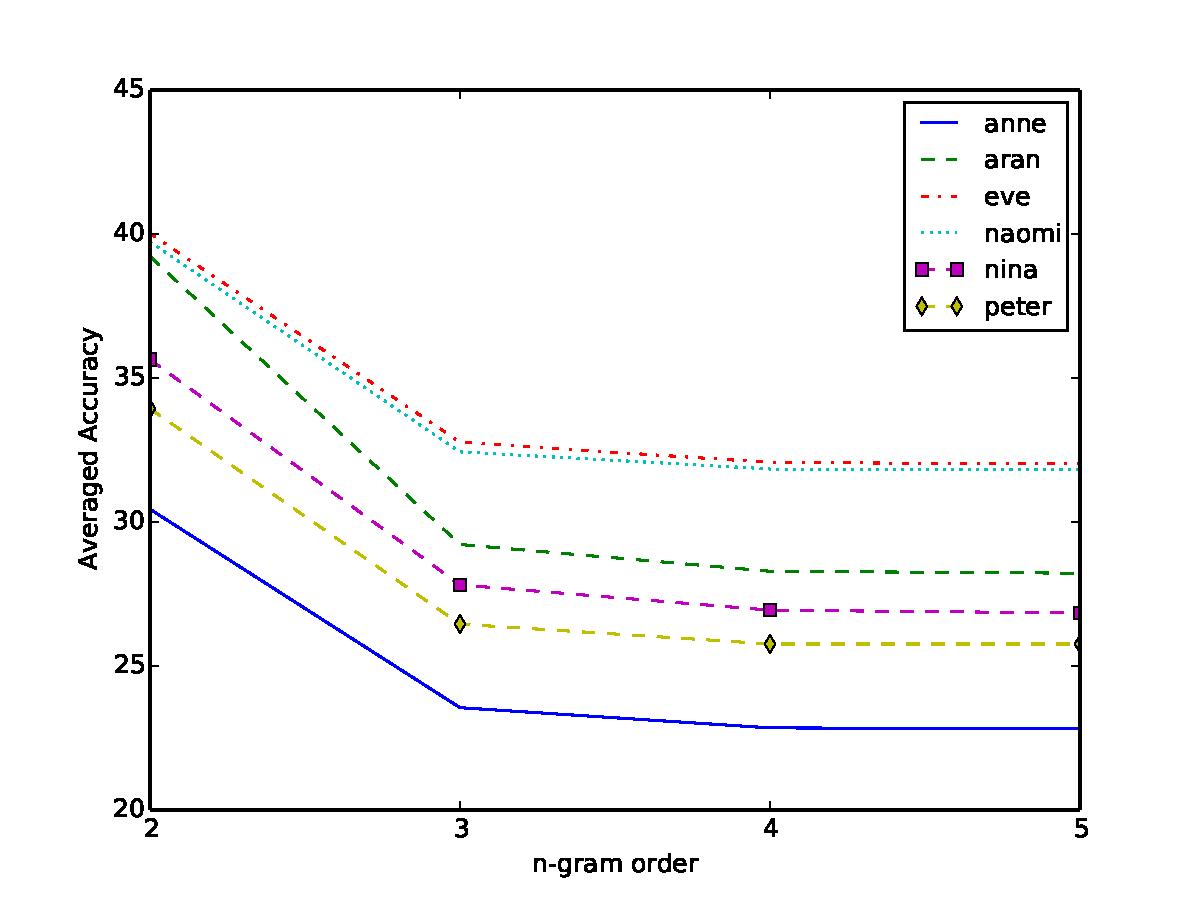
\includegraphics[width=.5\textwidth]{../figures/perplexity.pdf}
  \label{fig:perplexity}
  }
  \subfigure[]{
  \includegraphics[width=.5\textwidth]{../figures/ngram.pdf}
  \label{fig:ngram}
  }
  \caption{Language Model perplexities on each child corpus for different
  n-gram orders are presented on the left figure while 10-fold cross validation
  accuracies calculated based on these models are presented on the right.} 
\end{figure}

The perplexity of each child corpus is dramatically improved when the n-gram
order of the language model is increased from 2 to 3 and varies slightly for
orders higher than 3.  Figure~\ref{fig:perplexity} plots the perplexity versus
the n-gram order.  As shown in Figure~\ref{fig:ngram}, the model classification
accuracies on each child corpus are slightly improved for orders higher than 3
which is in fact parallel to the perplexity trends in
Figure~\ref{fig:perplexity}.  Overall, the classification accuracy of
paradigmatic model is highly correlated with the perplexity of the language
model that is used to sample substitutes.

%% One possible explanation of similar performances with n-grams 3,4 and 5 is
%% that our model defines the context of a target word by using $2n-2$ words
%% (i.e., $n-1$ words left to the target word and $n-1$ word right to the target
%% word) however most of the sentences in our test corpora is shorter than 7
%% words. 
%%% Presenting them with figure is much more powerful
%%% Perplexity of LM with different n-grams
%%\begin{table}[ht]
%%\centering
%%\caption{Language model perplexities on each child corpus for different n-gram
%%orders.} 
%%\begin{tabular}{lcccc}
%%  \hline  
%%  Child & 2-gram & 3-gram & 4-gram & 5-gram \\
%%  \hline
%%  Anne  & 30.44 & 23.55 & 22.85 & 22.81\\
%%  Aran  & 39.22 & 29.21 & 28.28 & 28.21\\
%%  Eve   & 40.02 & 32.77 & 32.06 & 32.01\\
%%  Naomi & 39.72 & 32.43 & 31.83 & 31.81\\
%%  Nina  & 25.64 & 27.81 & 26.93 & 26.84\\
%%  Peter & 33.93 & 26.45 & 25.76 & 25.76\\
%%  \hline
%%\end{tabular}
%%\label{t:perplexity}
%%\end{table}
%%
%%\begin{figure}[h]
%%  \subfigure[$aX$ model with $5K$ iterations] {
%%    \includegraphics[width=0.4\textwidth]{../figures/prtags5K.pdf}
%%    \label{fig:subfig5}
%%  }
%%  \subfigure[$Xb$ model with $5K$ iterations] {
%%    \includegraphics[width=0.4\textwidth]{../figures/pstags5K.pdf}
%%    \label{fig:subfig6}
%%  }
%%  \subfigure[$aXb$ model with $5K$ iterations] {
%%    \includegraphics[width=0.4\textwidth]{../figures/fretags5K.pdf}
%%    \label{fig:subfig7}
%%  }
%%  \subfigure[$aX+Xb$ model with $5K$ iterations] {
%%    \includegraphics[width=0.4\textwidth]{../figures/fletags5K.pdf}
%%    \label{fig:subfig8}
%%  }
%%  \subfigure[$a*b$ model with $5K$ iterations] {
%%    \includegraphics[width=0.4\textwidth]{../figures/wsubtags100K.pdf}
%%    \label{fig:subfig9}
%%  }
%%  \caption{10-fold cross validation individual tag accuracies of $aX$, $Xb$,
%%  $aXb$, $aX+Xb$ and $a*b$ on each child corpus after $5K$ iterations
%%  of feed-forward connectionist algorithm.}
%%  \label{fig:learningIteration5KApp}
%%\end{figure}
%%
%%\begin{figure}[h]
%%  \subfigure[$aX$ model with $100K$ iterations] {
%%    \includegraphics[width=0.4\textwidth]{../figures/prtags100K.pdf}
%%    \label{fig:subfig10}
%%  }
%%  \subfigure[$Xb$ model with $100K$ iterations] {
%%    \includegraphics[width=0.4\textwidth]{../figures/pstags100K.pdf}
%%    \label{fig:subfig11}
%%  }
%%  \subfigure[$aXb$ model with $100K$ iterations] {
%%    \includegraphics[width=0.4\textwidth]{../figures/fretags100K.pdf}
%%    \label{fig:subfig12}
%%  }
%%  \subfigure[$aX+Xb$ model with $100K$ iterations] {
%%    \includegraphics[width=0.4\textwidth]{../figures/fletags100K.pdf}
%%    \label{fig:subfig13}
%%  }
%%  \subfigure[$a*b$ model with $100K$ iterations] {
%%    \includegraphics[width=0.4\textwidth]{../figures/wsubtags100K.pdf}
%%    \label{fig:subfig14}
%%  }
%%  \caption{10-fold cross validation individual tag accuracies of $aX$, $Xb$,
%%  $aXb$, $aX+Xb$ and $a*b$ on each child corpus after $100K$ iterations
%%  of feed-forward connectionist algorithm.}
%%  \label{fig:learningIteration100KApp}
%%\end{figure}
% What happens when we change the data size?\\
% What happens when we change the vocabulary threshold?\\
% 
% \subsection{Input Corpora}
% \subsection{Method}
% \subsection{Results}
% 
% %% Let's drop this experiment, it is expensive.  We might handle 
% %% it hacking the fastsubs but I'm not sure about the mathematics.
% %% \section{Experiment 5}
% %% Left/rigth context substitute
% %% \subsection{Input Corpora}
% %% \subsection{Method}
% %% \subsection{Results}
% \section{Experiment 6}
% Other languages that we have in CHILDES
% 
% \section{Experiment 7}
% What happens if some of the words are given (semi-supervised setting)
% 
% \subsection{Input Corpora}
% \subsection{Method}
% \subsection{Results}




\section{General Discussion}

This study proposes paradigmatic representations of context as opposed to
syntagmatic representations for syntactic category acquisition. The
paradigmatic approach suggests to use probable substitutes of word ($a*b$). On
the other hand the syntagmatic approach proposes to use the preceding bigram
and the succeeding bigram whichever is fruitful ($aX + Xb$).

In order to contrast these two representations we replicate the experimental
setup of \cite{clair2010}. Experiments show that when the models exposed to
limited amount of training patters the $a*b$ is significantly more accurate
than $aX + Xb$. Results of long training phase show the same pattern, however,
the gap between these approaches gets smaller.

We investigate the dependency of the model to the number of substitutes. In
this experimental setup the number of substitutes varies from 1 to 64. The
results show that the accuracy of the model dramatically increases up to 16.
After 16 substitutes, no significant improvement in accuracy is observed. We
conclude that the model is robust as long as 16 substitutes are observed.

We explore the effect of the n-gram order of language model to the accuracy of
the model. While determining the probability of the next word in a sequence of
words, n-gram order determines how many preceding should be considered.  We
hypothesise that order of n-gram determines how accurate the substitutes of a
target word. Thus, it should affect the ($a*b$) model's accuracy.
Figure~\ref{fig:perplexity} and Figure~\ref{fig:perplexity} show that the
model's performance highly dependend on the n-gram order of the language model.

\appendix
\section{Preprocessing}
\label{app:preprocessing}
We apply following preprocessing steps initial to our analysis:
\begin{itemize}
\item All punctuation, pause, trailing off and interruption marks are
  treated as utterance boundaries.
\item Repetitions of a word are kept in the text and their grammatical
  categories are automatically set to the grammatical category of the
  original word.
\item Words that are grammatically necessary but not spoken are
  deleted (grammatical omissions).
\item Shortenings, dropping sounds out of words, are ignored and converted to
  the corresponding actual word forms.
\item Untranscribed words such as {\it xxx} or {\it yyy} are removed. 
\item Assimilations, complex sound changes of words or word phrases, are not
  converted to the actual form.
\end{itemize}

\section{Frequent Frames}
\label{app:mintz03}
In this section we replicated \cite{clair2010} to compare the amount of
categorical information provided by the top-45 fixed and bi-gram frames.

\begin{table}[ht]
  \footnotesize
  \centering
  \caption{Summary of the total number of utterances and types in each
    child corpus.  For the sake of space, we only report the percentages of
  analyzed utterances(types) in the top-45 $aXb$, $aX$ and $Xb$.}
  \begin{tabular}{lccccc}
    \hline
    Corpus & \specialcell{Corpus\\Utterances(Types)}&\multicolumn{3}{c}{\specialcell{Analyzed\\Utterances(Types)}}\\
    && $aXb$ & $aX$ & $Xb$ \\ 
    \hline
    Anne & 93371(2623) & .0462(.1357)& .3994(.8147) & .3619(.6465)\\ 
    Aran & 104997(3256)& .0537(.1901)& .4383(.8353) & .4026(.6670)\\ 
    Eve  & 59095(2184) & .0595(.1735)& .4097(.7770) & .3505(.5650)\\
    Naomi& 28793(1883) & .0572(.1603)& .3988(.7785) & .3455(.5586)\\
    Nina & 72879(2036) & .0842(.2249)& .4805(.8560) & .4028(.7062)\\
    Peter& 72834(2145) & .0671(.1762)& .4318(.8027) & .3770(.6317)\\
    \hline
  \end{tabular}
  \label{tab:corpusstat45}
\end{table}

\begin{table}[ht]
  \footnotesize
  \centering
  \caption{$aXb$} \begin{tabular}{lcccc}
    \hline
    Corpus & \specialcell{Token\\Accuracy} & \specialcell{Type\\Accuracy} &
    \specialcell{Token\\Completeness} & \specialcell{Type\\Completeness}\\
    \hline
    Anne  & .9693(.3909) & .8870(.4209) & .0756(.0221) & .0864(.0221)\\ 
    Aran  & .9527(.4166) & .8582(.4096) & .0794(.0221) & .0819(.0226)\\
    Eve   & .9731(.4935) & .8973(.4895) & .0645(.0222) & .0681(.0226)\\
    Naomi & .9496(.4858) & .8910(.4983) & .0650(.0219) & .0630(.0224)\\
    Nina  & .9615(.4782) & .8855(.4616) & .0787(.0221) & .0902(.0219)\\
    Peter & .9468(.4600) & .8615(.5249) & .0586(.0222) & .0739(.0217)\\
    \hline
  \end{tabular}
  \label{t:mintz03aXb}
\end{table}
%% aX
\begin{table}[ht]
  \footnotesize
  \centering
  \caption{$aX$} \begin{tabular}{lcccc}
    \hline
    Corpus & \specialcell{Token\\Accuracy} & \specialcell{Type\\Accuracy} &
    \specialcell{Token\\Completeness} & \specialcell{Type\\Completeness}\\
    \hline
    Anne  & .6348(.2654) & .5667(.3104) & .0850(.0219) & .0694(.0221)\\ 
    Aran  & .5939(.2582) & .5472(.3000) & .0791(.0220) & .0727(.0220)\\
    Eve   & .6775(.2735) & .5954(.2966) & .1002(.0221) & .0752(.0221)\\
    Naomi & .6509(.2754) & .5996(.3082) & .1017(.0220) & .0821(.0222)\\
    Nina  & .6809(.2877) & .6287(.3525) & .1073(.0220) & .0745(.0221)\\
    Peter & .6527(.2618) & .5043(.2715) & .1103(.0220) & .0715(.0221)\\
    \hline
  \end{tabular}
  \label{t:mintz03aX}
\end{table}
%% Xb
\begin{table}[ht]
  \footnotesize
  \centering
  \caption{$Xb$} \begin{tabular}{lcccc}
    \hline
    Corpus & \specialcell{Token\\Accuracy} & \specialcell{Type\\Accuracy} &
    \specialcell{Token\\Completeness} & \specialcell{Type\\Completeness}\\
    \hline
    Anne  & .4462(.2613) & .4048(.2920) & .0651(.0651) & .0426(.0426)\\ 
    Aran  & .4758(.2755) & .4142(.3045) & .0733(.0733) & .0443(.0443)\\
    Eve   & .4492(.2601) & .3960(.2851) & .0676(.0676) & .0470(.0470)\\
    Naomi & .4532(.2602) & .3717(.2764) & .0740(.0740) & .0438(.0438)\\
    Nina  & .4837(.2650) & .4530(.3375) & .0867(.0867) & .0458(.0458)\\
    Peter & .4368(.2617) & .3500(.2702) & .0744(.0744) & .0417(.0417)\\
    \hline
  \end{tabular}
  \label{t:mintz03Xb}
\end{table}
\section{Experiment \arabic{ExperimentCounter}: Corpus analysis}
\begin{table}[ht]
  \small
  \centering
  \caption{10-fold cross-validation classification accuracies of models based
    on flexible frames ($aX + Xb$) and substitutes ($a*b$) on each child corpus
    after 100K training patterns are summarized.  Standard errors are reported
    in parentheses.  Lambdas of $aX+Xb$ and $a*b$ are both tested against each
    other and zero association by using two tailed z-test.  All tests have
    $p<.001$.} \begin{tabular}{lccccc}
    \hline
    Corpus & \multicolumn{2}{c}{$aXb$} 
    && \multicolumn{2}{c}{$aX+Xb$}\\ 
    \cline{2-3}
    \cline{5-6}
    & Accuracy & $\lambda$ && Accuracy & $\lambda$\\
   \hline
    Anne  & .5416 (.0224)& .3099 (.0255) &&.7628 (.0075) & .6407 (.0124)\\
    Aran  & .5156 (.0215)& .2837 (.0120) &&.7337 (.0059) & .5977 (.0081)\\
    Eve   & .5370 (.0258)& .3209 (.0130) &&.7580 (.0068) & .6351 (.0083)\\
    Naomi & .5229 (.0244)& .2840 (.0220) &&.7316 (.0086) & .5892 (.0113)\\
    Nina  & .5636 (.0113)& .3287 (.0183) &&.7755 (.0040) & .6547 (.0075)\\
    Peter & .5661 (.0180)& .3541 (.0206) &&.7670 (.0071) & .6518 (.0088)\\
    \hline
  \end{tabular}
  \label{t:frame100K}
\end{table}





%% \section{General Discussion}
%% The Appendices part is started with the command \appendix;
%% appendix sections are then done as normal sections
%% \appendix

%% \section{}
%% \label{}

%% References
%%
%% Following citation commands can be used in the body text:
%%
%%  \citet{key}  ==>>  Jones et al. (1990)
%%  \citep{key}  ==>>  (Jones et al., 1990)
%%
%% Multiple citations as normal:
%% \citep{key1,key2}         ==>> (Jones et al., 1990; Smith, 1989)
%%                            or  (Jones et al., 1990, 1991)
%%                            or  (Jones et al., 1990a,b)
%% \cite{key} is the equivalent of \citet{key} in author-year mode
%%
%% Full author lists may be forced with \citet* or \citep*, e.g.
%%   \citep*{key}            ==>> (Jones, Baker, and Williams, 1990)
%%
%% Optional notes as:
%%   \citep[chap. 2]{key}    ==>> (Jones et al., 1990, chap. 2)
%%   \citep[e.g.,][]{key}    ==>> (e.g., Jones et al., 1990)
%%   \citep[see][pg. 34]{key}==>> (see Jones et al., 1990, pg. 34)
%%  (Note: in standard LaTeX, only one note is allowed, after the ref.
%%   Here, one note is like the standard, two make pre- and post-notes.)
%%
%%   \citealt{key}          ==>> Jones et al. 1990
%%   \citealt*{key}         ==>> Jones, Baker, and Williams 1990
%%   \citealp{key}          ==>> Jones et al., 1990
%%   \citealp*{key}         ==>> Jones, Baker, and Williams, 1990
%%
%% Additional citation possibilities
%%   \citeauthor{key}       ==>> Jones et al.
%%   \citeauthor*{key}      ==>> Jones, Baker, and Williams
%%   \citeyear{key}         ==>> 1990
%%   \citeyearpar{key}      ==>> (1990)
%%   \citetext{priv. comm.} ==>> (priv. comm.)
%%   \citenum{key}          ==>> 11 [non-superscripted]
%% Note: full author lists depends on whether the bib style supports them;
%%       if not, the abbreviated list is printed even when full requested.
%%
%% For names like della Robbia at the start of a sentence, use
%%   \Citet{dRob98}         ==>> Della Robbia (1998)
%%   \Citep{dRob98}         ==>> (Della Robbia, 1998)
%%   \Citeauthor{dRob98}    ==>> Della Robbia


%% References with bibTeX database:
\clearpage
\bibliographystyle{model5-names}
\bibliography{childes}

%% Authors are advised to submit their bibtex database files. They are
%% requested to list a bibtex style file in the manuscript if they do
%% not want to use elsarticle-harv.bst.

%% References without bibTeX database:

% \begin{thebibliography}{00}

%% \bibitem must have one of the following forms:
%%   \bibitem[Jones et al.(1990)]{key}...
%%   \bibitem[Jones et al.(1990)Jones, Baker, and Williams]{key}...
%%   \bibitem[Jones et al., 1990]{key}...
%%   \bibitem[\protect\citeauthoryear{Jones, Baker, and Williams}{Jones
%%       et al.}{1990}]{key}...
%%   \bibitem[\protect\citeauthoryear{Jones et al.}{1990}]{key}...
%%   \bibitem[\protect\astroncite{Jones et al.}{1990}]{key}...
%%   \bibitem[\protect\citename{Jones et al., }1990]{key}...
%%   \harvarditem[Jones et al.]{Jones, Baker, and Williams}{1990}{key}...
%%

% \bibitem[ ()]{}

% \end{thebibliography}

\end{document}

%%
%% End of file `elsarticle-template-harv.tex'.

